\documentclass{beamer}
\usepackage{graphicx}
\usepackage{url}
\usetheme{Copenhagen}
\usecolortheme{seahorse}

\title{Free and Open Source Software at CERN:\\
	Integration of Drivers in The Linux Kernel}
\author{%
	Juan David Gonz\'alez Cobas, Samuel Iglesias Gons\'alvez,\\
	Julian Howard Lewis, Javier Serrano, Manohar Vanga (CERN, Geneva),\\
	Emilio G. Cota (Columbia University, NY; formerly at CERN), \\
	Alessandro Rubini, Federico Vaga (University of Pavia)}
\date{ICALEPCS'2011}

\begin{document}


\begin{frame}
\titlepage
\end{frame}

\begin{frame}
\tableofcontents
\end{frame}

\begin{frame}{CERN Controls System Front End Computers (FECs)}

The controls system relies on FECs on several form factors/buses,
most of them based on Single-Board Computers (SBCs)

\begin{itemize}
\item Number of FECs: 1140
\item Number of VME crates: 710
\end{itemize}

For the VME crates, the ongoing renovation process gives
\begin{itemize}
\item CES RIO2/RIO3 SBCs with PowerPC CPUs runing
LynxOS (around 605 crates by August 2011), to
\item MEN-A20 SBCs with Intel CPUs running real-time
Linux (around 105 by August 2011).
\end{itemize}
\end{frame}


\begin{frame}{MEN A20 and the TSI148 chip and driver}

The MEN A20 SBC is an Intel Core 2 Duo-based board interfacing to the
VME bus via a Tundra TSI148 PCI-X to VME bridge chip.

% wget http://www.men.de/docs-ext/products/images/img_photo/01a020-_hi.jpg
% ftp://ftp.ruby-lang.org/pub/ruby/1.8/ruby-1.8.7-p352.tar.gz
\begin{center}
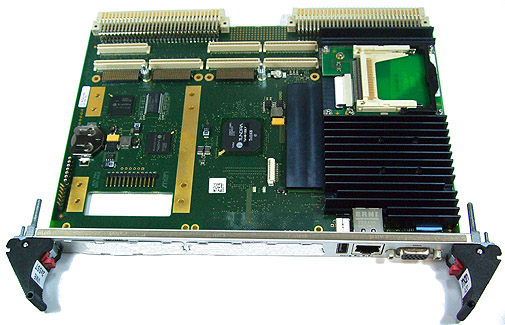
\includegraphics[height=4cm]{01a020-_hi.pdf} \qquad
\includegraphics[height=2.75cm]{p_tundra_Tsi148-HR.pdf}
\end{center}
\end{frame}


\section*{Outline}
\begin{frame}
\tableofcontents
\end{frame}
\section{Introduction}
\subsection{Overview of the Beamer Class}
\subsection{Overview of Similar Classes}
\section{Usage}
\subsection{...}
\subsection{...}
29
\section{Examples}
\subsection{...}
\subsection{...}
\begin{frame}
\end{frame} % to enforce entries in the table of contents
\end{document}

\iffalse



%%   VARIABLE HEIGHT FOR THE TITLE BOX (default 35mm)
\setlength{\titleblockheight}{48mm}

\title{%
    FREE AND OPEN SOURCE SOFTWARE AT CERN:\\
    INTEGRATION OF DRIVERS IN THE LINUX KERNEL}
\author{%
	Juan David Gonz\'alez Cobas, Samuel Iglesias Gons\'alvez,\\
	Julian Howard Lewis, Javier Serrano, Manohar Vanga (CERN, Geneva),\\
	Emilio G. Cota (Columbia University, NY; formerly at CERN), \\
	Alessandro Rubini, Federico Vaga (University of Pavia)}

\begin{document}

\maketitle
\begin{abstract}
    Most device drivers written for accelerator control systems suffer from a
    severe lack of portability due to the \emph{ad hoc} nature of the code,
    often embodied with intimate knowledge of the particular machine it is
    deployed in.
    In this paper we challenge this practice by arguing for the opposite
    approach: development \emph{in the open}, which in our case translates
    into the integration of our code within the Linux kernel. We make our
    case by describing the upstream merge effort of the \texttt{tsi148}
    driver, a critical (and complex) component of the control system.
    The encouraging results from this effort have then led us to follow the
    same approach with two more ambitious projects, currently in the works:
    Linux support for the upcoming FMC boards~\cite{fpga-fmc,vita-fmc}
    and a new I/O subsystem.
\end{abstract}


\section{TSI148 DRIVER INTEGRATION IN THE KERNEL}
\subsection{Rationale}
The VME bus is a central component of the Controls System at CERN. We rely
on 1140 FECs (Front End Computers), 710 of which are VME crates with SBC
(Single Board Computers). A process of renovation is in course, involving
the migration from
\begin{Itemize}
\item CES RIO2/RIO3 SBCs with PowerPC CPUs runing LynxOS (around 605
    crates by August 2011), to
\item MEN-A20 SBCs with Intel CPUs running real-time Linux (around 105 by
    August 2011).
\end{Itemize}

The MEN-A20 SBC incorporates a TSI148 VME-to-PCI-X bridge chip.  To support
the functionalities required, and for maximum backward compatibility with
the legacy CES API, a device driver was developed by CERN's BE/CO group in
spring 2009. Clearly, this is a critical component of the controls system:
every VME device relies on the provided programming interface to the VME
bus. The CERN-developed driver offers, therefore, a CES compatibility API
to facilitate the transition during the renovation process and a new API
more in line with what is common practice in the Linux kernel.

Work on the inclusion of the driver in the Linux kernel started in late
2010 and is currently nearing completion. This effort, along with its
motivations and consequences, is documented in the remainder of this
Section.

\subsection{Benefits}

There are many reasons that make the insertion of code in the mainline kernel
a desirable target.

\begin{Itemize}
\item Smoother maintenance in the (frequent) event of kernel API
  changes.~\cite{stable-api-nonsense}
\item Very strict process of peer review of the code by knowledgeable
    and specialised maintainers.
\item Widespread distribution of the code base, which can then be
    enhanced and get contributions by researchers working on similar
    problems.
\item Input from the topmost experts in the field.
\item Best practice and use of bleeding-edge tools selected by
    experienced programmers, \emph{e.g.} git~\cite{git}, sparse~\cite{sparse}
    and Coccinelle~\cite{coccinelle}.
\item Avoidance of suboptimal, \emph{ad hoc} solutions in favour of the
    best ones from the technical point of view.
\item Contributing back in return to the many benefits the FOSS community
    gives us.
\item Being able to drive a critical hardware component with software
    in the vanilla kernel, with no local, idiosyncratic modifications.
\end{Itemize}

It is worth noting that the importance of the last point only became
apparent once the merge effort was well underway. In our control system,
renovated FECs are \emph{diskless} machines that boot a custom \emph{rt}
kernel~\cite{linux-rt}, carefully configured and patched to match local
needs.  The upstream merge of the \emph{tsi148} driver allows us to deploy
off-the-shelf kernels packaged by linux distributions, thus largely reducing
the kernel maintenance burden.

\subsection{Caveats}

Some of the caveats herewith enumerated will be elaborated further in
the description of the integration process, but we summarize here the most
important ones.

\begin{Itemize}
\item It is hard, frustrating at times. One should be ready for the
    peculiar culture of the Linux Kernel Mailing List.
\item Design, APIs and coding practice that are customary or simply
    acceptable locally must be adapted or rebuilt to comply with the strict
    standards imposed by the Linux kernel developers. The morale is that
    the end product will most certainly be different to (and better than)
    the original.
\item One must be prepared to compromise. The most practical,
    short-lived solution might not be the technically perfect one kernel
    maintainers aim at.
\item Maintainers are occasionally hard to deal with.
\item The review process may be long; several iterations are usually
    necessary when merging significant changes.
\item Small, incremental changes are more likely to be accepted than
    big, hard-to-digest ones. The rule of thumb is to ``Separate \emph{logical
    changes} into a single patch file.''~\cite{submitting-patches}
\item Having a good history of prior contributions gives more respectability
    and ease of acceptance: the system is based on meritocracy.
\end{Itemize}

\subsection{The process}

Submission of source code for acceptance in the kernel is done by means of
patches subject to a process of peer review before acceptance. The reviews
are sometimes daunting, and much editing and re-submissions can result. This
process of strict code review is another good practice our team adopted for
its development process, a practice that has proved very beneficial.

Our fist attempt of integration of the \verb|tsi148| driver was initiated
in late 2010 by one of the authors (Emilio G. Cota).

By that time, a \verb|tsi148| driver had recently been admitted in
the \texttt{staging}~\cite{staging} area of the kernel, its maintainer being
Martyn Welch. This driver brought a tentative support for the VME bus that
covered two VME-to-PCI bridges:

\begin{Itemize}
\item The Tundra Universe chips, with work derived from VMELinux by John
Huggins and Michael Wyrick.
\item The Tundra TSI148 chip, inspired in the above.
\end{Itemize}

The set of patches initially submitted provided improvements in several areas,
esp. in orthodox implementation of the Linux bus/device model concepts.
Acceptance by the maintainer was partial, and modifications related to the
device model implementation remained controversial and not accepted.

In 2011, another of this paper's authors, Manohar Vanga, took over the
submission effort. Some bugs in the staging driver were fixed, and the bulk
of modifications concerning the device model were partially acknowledged. This
led to several review iterations; at the time of this writing, the definitive
submission and acceptance of the last set of patches concerning the core
device model is in its final stage, and will be applied by the corresponding
kernel maintainer in the next merge window.

Although the whole set of patches concerning bug fixes and device model of the
\verb|tsi148| VME bridge driver is finally accepted, there is still a long
way before reaching the final desideratum, \emph{i.e.,} driving our
\verb|tsi148| devices with stock software from the mainline kernel tree.
\begin{Itemize}
\item The outstanding goal should be now getting the VME driver out of the
\verb|./staging/| tree. For this to happen, the overall quality of the code must improve significantly.~\cite{staging}
\item There are API  incompatibilities with the driver currently used at
CERN; this implies that a transient kernel module must adapt interfaces
if driver code has to remain untouched.
\end{Itemize}

\section{DRIVERS FOR THE FMC FAMILY}

\begin{figure}[t]
   \centering
   \includegraphics*[width=80mm]{THCHMUST04f1.eps}
   \caption{Wishbone bus driver architecture}
   \label{wishbone-enum}
\end{figure}

A family of carrier/mezzanine modules compliant with the ANSI VITA~57
FMC standard~\cite{vita-fmc} is described in~\cite{fpga-fmc}. This kit
of boards, developed by the BE/CO Hardware and Timing section at CERN is
another case in point for the benefits of a Linux kernel-centric
approach. The hardware concept
and architecture are described in the aforementioned paper~\cite{fpga-fmc}; the
key point is that the mezzanine provides basic circuitry, and the core of the
application logic is implemented in the FPGA of the carrier board. The cores
inside this FPGA are interconnected via a Wishbone~\cite{wishbone-spec} bus.


From the software point of view, a particular instance of this family
behaves like a PCI-to-Wishbone or VME-to-Wishbone bridge. The Wishbone
bus interconnects a set of cores providing functionalities that are either
common to the whole family of mezzanines, or specific to the application
board actually plugged in the FMC slot. We show in figure~\ref{slow-adc}
the block diagram of the FMC 100MS 14 bit ADC, a typical example of an FPGA
application comprising cores for, among others

\begin{Itemize}
\item Basic I${}^2$C interfacing to the mezzanine board.
\item Wishbone mastering.
\item DMA access to DDR3 memory in the carrier board.
\item Mezzanine-specific control logic (\emph{e.g.} ADC programming/setup).
\item Interrupt control.
\end{Itemize}
The consequence of this modular design of the application FPGA is that
the device driver architecture reflects the structure of this set of cores
(see figure~\ref{wishbone-enum}). The driver for the carrier board performs
essentially the following basic functions
\begin{Itemize}
\item Identify the carrier board and initialize it.
\item Perform a basic identification of the mezzanine(s) installed in
    the FMC slot(s), and their configured applications.
\item Load the application firmware into the carrier FPGA.
\item Register a Wishbone bus with the kernel.
\item Enumerate the cores in that firmware (to wit, the
    inner blocks in figure~\ref{slow-adc}).
\item Register the devices those cores implement and install the drivers
    associated to them.
\end{Itemize}
The process is directly implied by how the Linux kernel device model
is implemented as described in~\cite{device-model} or in chapter~14
of~\cite{rubini}. Conceptually, it amounts to the provision of a bus driver
for Wishbone, plus a PCI-to-Wishbone bridge driver for the carrier board.

\begin{figure}[t]
   \centering
   \includegraphics*[width=80mm]{THCHMUST04f2.eps}
   \caption{Block diagram of the FMC slow ADC application}
   \label{slow-adc}
\end{figure}

Modularity and reusability of cores and drivers are not the only rationale
behind this design. Actually, the drivers for the FMC family are the second
family of drivers planned to be integrated in the mainline kernel. Given
that boards and their applications will be manufactured by external
companies and available to the general public and not only to CERN,
having their drivers and the Wishbone
bus integrated upstream is the logical step to take. The Wishbone enumeration is made
possible through the definition of an FPGA configuration space developed
in~\cite{fpga-config-space}, that will be the basis for the integration of
all drivers of this family in the kernel.

\section{DATA ACQUISITION DRIVERS: KERNEL FRAMEWORKS}

The third family of drivers considered for integration upstream is less
homogeneous than the FMC family. The BE/CO group supports a standard kit
of hardware modules for data acquisition and general analog and digital I/O,
some of whose characteristics can be compared in table~\ref{zio-modules}. Linux
drivers for these modules were developed in different stages of the renovation
process, leading from legacy LynxOS drivers to Linux; therefore, there is a
varying degree of adherence to standard practice among the Linux kernel
developers,
because of the LynxOS coding practice formerly prevalent.

\begin{table*}[ht]
   \centering
   \caption{BE/CO data acquisition modules}
   \begin{tabular}{llllll}
       \toprule
	\textbf{Module}& \textbf{Type}& \textbf{Channels}&
	\textbf{Resolution}& \textbf{Max. Speed}& \textbf{Bus} \\
       \midrule
	VMOD-12E8/16    &  Analog input  & 8/16ch & 12b    & 15us/sample & VME/PCI  \\
	VD80            &  Analog input  & 16ch   & 16b    & 200kS/s     & VME  \\
	SIS3300         &  Analog input  & 8ch    & 12/14b & 100MS/s     & VME  \\
	SIS3302         &  Analog input  & 8ch    & 16b    & 100MS/s     & VME  \\
	SIS3320         &  Analog input  & 8ch    & 12b    & 250MS/s     & VME  \\
	``Fast'' FMC ADC&  Analog input  & 4ch    & 14b    & 100Ms/s     & VME/PCIe (Wishbone)  \\
	``Slow'' FMC ADC&  Analog input  & 8ch    & 16b    & 100kS/s     & VME/PCIe (Wishbone)  \\
       \midrule
	CVORB V4        &  Analog output & 16ch   &  16b   &  5us/sample & VME 	 \\
	VMOD-12A2/4     &  Analog output & 2ch    &  12b   &  10us/sample& VME/PCI \\
	CVORG           &  Analog output & 2ch    &  14b   &  100 MS/s   & VME  \\
       \midrule
	VMOD-TTL        &  Digital I/O   & 20ch   & 1b     & n/a         & VME/PCI \\
	CVORA           &  Digital I/O   & 32ch   & 1--32b & 100Mhz	 & VME \\
       \bottomrule
   \end{tabular}
   \label{zio-modules}
\end{table*}

Two needs arise here clearly, in the light of our intention of having our
whole set of drivers incorporated upstream:
\begin{Itemize}
\item Proceed to a more homogeneous, Linux-only code base.
\item Provide a general framework for data acquisition and control
    devices.
\end{Itemize}
Concerning the latter, there are two candidate Linux kernel frameworks:
Comedi~\cite{comedi} and IIO~\cite{iio}. Both are in \texttt{./staging/}, and
careful analyses show that they prove insufficient for our needs. Therefore,
the development of a more complete and acceptable framework for industrial data
acquisition and analog/digital I/O becomes part of our effort of integrating
our supported device drivers in the Linux kernel. This effort is motivated
both by the requirements of legacy drivers and by the requirements that
the FMC family will impose in driver design, esp. in the area of operating
system interface.

Such a framework, codenamed \texttt{zio}, intends to cover all the relevant
aspects of data acquisition devices, far beyond the existing frameworks,
such as
\begin{Itemize}
\item Digital and analog input and output.
\item One-shot and streaming (buffered) data acquisition or waveform play.
\item Resolution.
\item Sampling rate.
\item Buffer management and timing for streaming conversion.
\item Support for DMA.
\item Calibration, offset and gain.
\item Bit grouping in digital I/O.
\item Timestamping.
\item Triggering of acquisition/output.
\item Clean design conforming to Linux kernel practice.
\end{Itemize}
At the time of this writing, prototype versions of the framework software
are under development phase~\cite{zio-git}.

\section{FORTHCOMING STRATEGY}

The strategy for inclusion of our driver kit in the kernel relies now on a
handful of key milestones
\begin{Enumerate}
\item Initiate upstream integration of the Wishbone bus driver.
	\label{wb}
\item Make the in-tree and our local API for \verb|tsi148| converge.
	\label{api}
\item Get the VME driver out of \texttt{staging}.
\item Develop the \texttt{zio} framework as a competitive alternative
	to Comedi and IIO.
	\label{zio}
\item Initiate integration of the \texttt{sis33xx} drivers into the
    \texttt{zio} framework and the mainstream kernel.
\end{Enumerate}
Points~\ref{wb}, \ref{api} and~\ref{zio} are short-term priorities that
should come out as quite straightforward.

\section{LESSONS LEARNED}

The main lessons we got from this process, that we will have to take into
account in the course of the forthcoming integrations, are
\begin{Itemize}
\item Being there first gives competitive advantage. However technically
    sound a proposal might be, it is better to get it accepted when it is new,
    and not contending with other more entrenched positions.
\item Getting input and enhancements from Linux peer developers
    is tremendously beneficial to improve the quality of the code, of the
    design and of the working environment (tools, policies and style being
    naturally given by what the Linux kernel developers have already tried
    and tested over many years).
\item
    There is a change of thinking when it comes to development after a while
    in the kernel community. The mindset changes from thinking of the short
    term goals to thinking of solutions that can scale to a larger set of
    problems. One starts to think of more generic solutions rather than
    quickly hacking together the fastest solution to the problem at hand.
\end{Itemize}

\section{CONCLUSIONS}

Contrary to what conventional assumptions dictate, low-level software
and development need not be intimately linked to, nor closely shaped
after, the peculiarities of a single control system. Developing with a
wider scope in mind is possible, as our experience proves. But not only
that: it results in technically superior, more scalable and maintainable
solutions.

Last, but not least, peer review, advice and a bleeding-edge set of tools
created by top level programmers contribute to the efficiency and quality
of the development process; a priceless gift we also owe to the
community of Linux kernel developers.

% \begin{thebibliography}{9}   % Use for  1-9  references
\begin{thebibliography}{99} % Use for 10-99 references

\bibitem{fpga-fmc}
P. Alvarez, M. Cattin, J. H. Lewis, J. Serrano and T. Wlostowski,
``FPGA Mezzanine Cards for CERN’s Accelerator Control System'',
in ICALEPCS'09, p. 376, 2009.

\bibitem{vita-fmc}
VME International Trade Association,
``FPGA Mezzanine Card (FMC) Standard'', \url{http://www.vita.com/}

\bibitem{wishbone-spec}
OpenCORES,
``Wishbone B4: WISHBONE System-on\-{}{}Chip (SoC) Interconnection
Architecture for Portable~IP Cores'', see\\
\url{http://opencores.org/opencores,wishbone}

\bibitem{git}
L. Torvalds. ``git: The Fast Version Control System'', see\\
\url{http://git-scm.com/}.

\bibitem{sparse}
L. Torvalds. ``Sparse - a Semantic Parser for C'', see\\
\url{http://sparse.wiki.kernel.org/}.

\bibitem{coccinelle}
J.L. Lawall, J. Brunel, N. Palix, R.R. Hansen, H. Stuart, G. Muller,
``WYSIWIB: A declarative approach to finding API protocols and bugs in
Linux code,'', in The 39th Annual IEEE/IFIP International Conference on
Dependable Systems and Networks, pp. 43-52, 2009.

\bibitem{device-model}
``Linux Kernel Device Model'', see\\
\texttt{linux-src/Documentation/driver-model/.}

\bibitem{stable-api-nonsense}
G. Kroah-Hartman, ``The Linux Kernel Driver Interface'', see Linux
sources under\\
\texttt{Documentation/stable\_api\_nonsense.txt.}

\bibitem{linux-rt}
S. Rostedt and D.V. Hart, ``Internals of the RT patch''. In Linux
Symposium, 2007.

\bibitem{submitting-patches}
``Submitting Patches'', see\\
\texttt{linux-src/Documentation/SubmittingPatches.}

\bibitem{staging}
G. Kroah-Hartman, ``linux-staging tree created'', announcement on the
Linux Kernel Mailing List, June 2010.
See \url{https://lkml.org/lkml/2008/6/10/329}

\bibitem{rubini}
J. Corbet, A. Rubini, G. Kroah-Hartman, ``Linux Device Drivers'', 3rd
edition. 2005.

\bibitem{fpga-config-space} FPGA config space Open Hardware
Project, see
\url{http://www.ohwr.org/projects/fpga-config-space/}

\bibitem{comedi} See \url{http://www.comedi.org/}
\bibitem{iio} See article in \url{http://lwn.net/Articles/339674/}
\bibitem{zio-git} See \url{git://gnudd.com/zio-beta.git}

\end{thebibliography}

\end{document}
\if
